\documentclass[../main.tex]{subfiles}
\graphicspath{{\subfix{../images/}}}
\begin{document}

Duální báze k $\mathcal{N} = (N_1, ... , N_d) \text{ v } \mathcal{P}: (\Phi_1, ..., \Phi_d)$, kde $N_i(\Phi_j) = \delta_{ij}$

\subsection{Příklady:}

\subsubsection{1D prvek s nejvýše lineárními polynomy:}
$K = (0,1), \mathcal{P} = \{  v: <0,1> \mapsto \mathbb{R} | v(x) = a + bx, a,b \in \mathbb{R}       \} \implies dim(\mathcal{P}) = 2 \implies \mathcal{N} = (N_1, N_2)$

Proto zvolíme: $N_1(v) = v(0), N_2(v) = v(1)$

\begin{lemma}
    Pak $(K, \mathcal{P}, \mathcal{N})$ je KP
\end{lemma}
\begin{proof}
    \begin{itemize}
        \item $K = (0,1)$ je omezená oblast v $\mathbb{R}$ $\checkmark$
        \item $\mathcal{P}$ má dimenzi 2 $\checkmark$
        \item Je $\mathcal{N}$ báze $\mathcal{P}^\#$ ? tj LN?: \hfill \break
            Nechť $v_0(x) = a+bx$ je libovolný, $\implies (N_1(v_0) = v_0(0) = a) \wedge N_2(v_0) = v_0(1) = a + b$ a nechť $N_1(v_0) = 0 \wedge N_2(v_0) = 0$  \hfill \break
            $\implies (a=0) \wedge (a+b = 0) \implies a=b=0 \implies v_0(x) = 0 \implies (N_1, N_2)$ je LN $\checkmark$

    \end{itemize}        
\end{proof}
\begin{definition}
    Tento prvek nazýváme jako tzv. lineární Lagrangeův prvek
\end{definition}


\begin{definition}[Duální (uzlové) báze]

    $N_i(\Phi_j) = \delta_{ij}$ označme $\Phi_i(x) = a_i + b_i x, i = 1,2\implies$
    
    \todo{Highlight prave s \ hl strany + align}
    \begin{multline}
        N_1(\Phi_1) = 1 (\Phi_1(0) = 1) : a_1 = 1 \hfill  N_1(\Phi_2) = 0 (\Phi_2(0) = 0): a_2 = 0 \\
        N_2(\Phi_1) = 0 (\Phi_1(1) = 0) : a_1 + b_1 = 0 \hfill N_2(\Phi_2) = 1 (\Phi_2(1) = 1): a_2 + b_2 = 1    
    \end{multline}
    Zapišme dohromady že se zvýrazněné strany rovnají. 

    \begin{gather}
    \left(\begin{array}{cc|cc}
        1 & 0 & 1 & 0 \\
        1 & 1 & 0 & 1 
    \end{array}\right)
    \sim
    \left(\begin{array}{cc|cc}
        1 & 0 & 1 & 0 \\
        0 & 1 & -1 & 1 
    \end{array}\right)
    \implies
    \begin{array}{c}
        \Phi_1(x) = 1 - x  \\
        \Phi_2(x) = x
    \end{array}
\end{gather}

    \begin{figure}[ht]
        \centering
        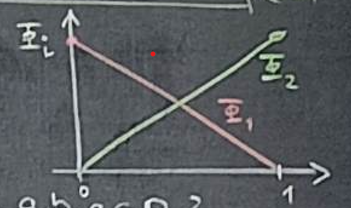
\includegraphics{images/vzhled1dlagrangeprvku.png}
        \caption{Vzhled 1D Lagrangeovského prvku}
    \end{figure}
\end{definition}


\subsubsection{1D prvek s nejvýše kvadratickými polynomy:}
$K = (0,1), \mathcal{P} = \{  v: <0,1> \mapsto \mathbb{R} | v(x) = a + bx + cx^2, a,b,c \in \mathbb{R}       \} \implies dim(\mathcal{P}) = 3 \implies \mathcal{N} = (N_1, N_2, N_3)$
Například zvolme $N_1(v) = v(0), N_2(v) = v(1), N_3(v) = v(\frac{1}{2})$

\begin{lemma}
    $(K, \mathcal{P}, \mathcal{N})$ je KP
\end{lemma}
\begin{proof}
    \begin{itemize}
        \item $K = (0,1)$ je omezená oblast v $\mathbb{R}$ $\checkmark$
        \item $\mathcal{P}$ má dimenzi 3, obsahuje polynomy $\checkmark$
        \item Je $\mathcal{N}$ báze $\mathcal{P}^\#$ ? tj LN?: \hfill \break
            Nechť $v_0(x) = a+bx+cx^2$ je libovolný, v situaci $N_1(v_0) = 0 \wedge N_2(v_0) = 0 \wedge N_3(v_0) = 0$ máme \hfill \break
            $\implies (a=0) \wedge (a+b+c = 0) \wedge (a+\frac{1}{2}b + \frac{1}{4}c = 0) \implies a=b=c=0 \implies (N_1, N_2, N_3)$ je LN $\checkmark$
    \end{itemize}        
\end{proof}
\begin{definition}
    Toto nazýváme kvadratickým Lagrangeovským prvkem.
\end{definition}


\begin{definition}[Duální báze]
Chceme $N_i(\Phi_j) = \delta_{ij}$, označme $\Phi_i(x) = a_i + b_ix + c_ix^2$.
Dostáváme následující rovnice.
\begin{multline}
    \Phi:  a_1 = 1                                 \Phi_2:    a_2 = 0                                 \Phi_3:    a_3 = 0             \\
            a_1 + b_1 + c_1 = 0                                 a_2 + b_2 + c_3 = 1                                 a_3 + b_3 + c_3 = 0 \\
            a_1 + \frac{1}{2}b_1 + \frac{1}{4}c_1 = 0           a_2 + \frac{1}{2}b_2 + \frac{1}{4}c_2 = 0           a_1 + \frac{1}{2}b_1 + \frac{1}{4}c_1 = 1
\end{multline}
Zapišme tento systém jako matici:

\todo{matice}

Dostáváme následující:
\begin{equation}
    \Phi_1(x) = 1-3x+2x^2, \Phi_2(x) = -x + 2x^2, \Phi_3(x) = 4x - 4x^2 
\end{equation}

\begin{figure}[ht]
    \centering
    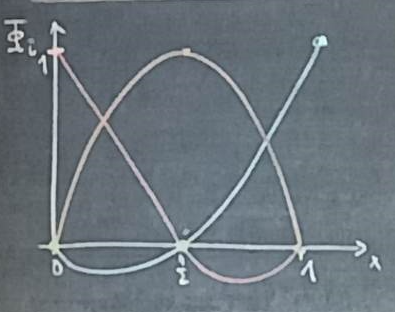
\includegraphics{images/vzhled1dlagrangeprvkukvadraticky.png}
    \caption{Vzhled 1D kvadratického Lagrangeovského prvku}
\end{figure}

\end{definition}

\begin{remark}
    Pro vlastnost 3. jsme použili kritérium LN v $\mathcal{P}^\#$ \break
    $(N_1, ..., N_d)$ je LN $<=> \left[  (\forall v_0 \in \mathcal{P})(\forall j \in \{1,...,d\})(N_j(v_0) = 0) \implies v_0 \equiv 0       \right]$\todo{maybe fix the last 0} 
\end{remark}


\begin{remark}
    Budeme využívat zužování polynomů na lineární nadplochy v $\mathbb{R}^n$ popsatelné pomocí lineárních funkcionálů: \break
    $M \subset \mathbb{R}^n$ je lineární nadplocha $<=> (\exists \alpha\in \mathbb{R})(\exists f \in (\mathbb{R}^n)^\#)(M\equiv \left\{ x\in\mathbb{R} | f(x) = \alpha    \right\})$ \break
    Pro jednoduchost níže zvolíme $\alpha = 0$ (Případným posunem počátku souřadnic)
\end{remark}

\begin{lemma}[O redukci]
    Nechť $\mathcal{P}$ je polynom stupně $\mathcal{D} \geq 1$ v $n$ proměnných, který je roven $0$ v nadrovině $V$, která je popsána funkcionálem $L\in(\mathbb{R}^n)^\#$ (tj. $V\equiv \left\{x\in\mathbb{R}^n| L(x)= 0\right\}$).
    Pak existuje polynom $Q$ stupně $\mathcal{D} - 1$ tak, že $(\forall x\in\mathbb{R}^n)(P(x) = L(x)*Q(x))$    
\end{lemma}

\begin{proof}
    Záměna proměnných tak, že $L(x) = L(\hat{x}, x_n) = x_n$ (kde $\hat{x} = [x_1,...,x_{n-1}]$), pak $V\equiv x_n = 0$

    Pak $P(x) = P(\hat{x},x_n) = \sum_{j=0}^\mathcal{D} \sum_{|\hat{j}| = 0}^{\mathcal{D}-j} c_{\hat{j}j}\cdot\hat{x}^{\hat{j}}\cdot x_n^j$ 
    kde $\hat{j}=\left[j_1,...,j_{n-1}\right], |\hat{j}| = \sum_{k=1}^{n-1}j_k$, $\hat{x}^{\hat{j}} = \prod_{l=1}^{n-1}x_l^{j_l}$

    Z podmínky $P|_V = 0 \implies P|_V = P(\hat{x},0) = \sum_{j=0}^\mathcal{D} \sum_{|\hat{j}| = 0}^{\mathcal{D}-j} c_{\hat{j}j}\cdot\hat{x}^{\hat{j}}\cdot 0^j$    $\implies\sum_{|\hat{j}| = 0}^{\mathcal{D}-j} c_{\hat{j}0}\cdot\hat{x}^{\hat{j}}\equiv0, \forall\hat{x}\in\mathbb{R}^{n-1}$

    $\implies c_{\hat{j}0} = 0 \forall j$

    $\implies P(\hat{x},x_n) = \sum_{j=1}^\mathcal{D} \sum_{|\hat{j}| = 0}^{\mathcal{D}-j} c_{\hat{j}j}\cdot\hat{x}^{\hat{j}}\cdot x_n^j = x_n \sum_{j=1}^\mathcal{D} \sum_{|\hat{j}| = 0}^{\mathcal{D}-j} c_{\hat{j}j}\cdot\hat{x}^{\hat{j}}\cdot x_n^{j-1}$

    $x_n$ je námi hledané $L(x)$, zbytek označme jako $Q(x)$
\end{proof}

\section{Nejpoužívanější typy konečných prvků}
\begin{remark}
    Ukážeme v $\mathbb{R}^2$, $\mathcal{K}$ bude simplex s vrcholy $z_1, z_2, z_3$.

    Lineární polynom v $\mathbb{R}^2 : v_0(x_1,x_2) = a + bx_1 + cx_2 $ 
    Kvadratický polynom v $\mathbb{R}^2 : v_0(x_1,x_2) = a + bx_1 + cx_2 + dx_1^2 + ex_1x_2 + fx_2^2 $
\end{remark}

\begin{figure}[ht]
    \centering
    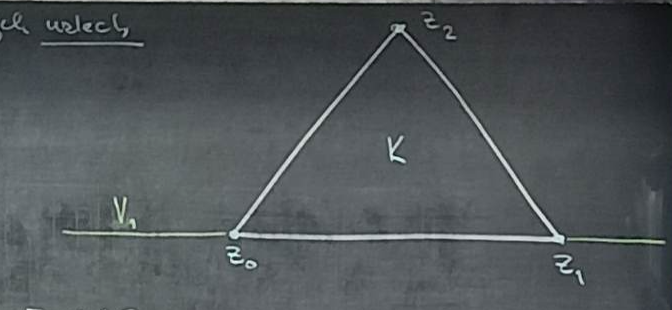
\includegraphics{images/simplex3uzly.png}
    \caption{Simplex ve 2D}
\end{figure}

\subsection{Lagrangeův prvek}
Uzlové proměnné poskytují hodnoty funkcí v $\mathcal{P}$ ve vybraných uzlech

\subsubsection{Lineární Lagrangeův prvek}
$\mathcal{P}$ obsahuje nejvýše lineární polynomy v $\mathbb{R}^n$

\begin{itemize}
    \item $K$ je simplex $\checkmark$
    \item $\mathcal{P}$ má dimenzi 3 $\checkmark$
    \item Jako bázi $\mathcal{N}$ navrhneme  $N_1(v)=v(z_0), N_2(v) = v(z_1), N_3(v)=v(z_2)$
\end{itemize} 

\begin{lemma}
    Pak $(K, \mathcal{P}, \mathcal{N})$ je KP
\end{lemma}
\begin{proof}
       Ukážeme LN $(N_1,N_2,N_3)$ pomocí kritéria výše:

       Nechť pro všechna $v\in\mathcal{P}: N_j(v) = 0, j\in\{1,2,3\}\implies v(z_j)=0$
       
       Argument jedné proměnné:

       Protože $v(z_0)=0\wedge v(z_1)=0 \wedge v\in\mathcal{P}$ je lineární polynom $\implies v|_{V_1}$ je lineární polynom jedné proměnné

       tj: $V_1 \equiv  \begin{cases}
        x_1(s) &= z_0^1 + (z_1^1 - z_0^1)s \\
        x_2(s) &= z_0^2 + (z_1^2 = z_0^2)s 
    \end{cases}, s\in\mathbb{R}
    \implies v|_{V_1} = v(x_1(s), x_2(s))$ je lineární polynom proměnné $\underline{s}$, přitom se rovná $0$ pro $ s=0,1$

    $\implies v|_{V_1}\equiv 0$ všude na $V_1$

\end{proof}

\begin{lemma}[Redukční lemma]
    $v(x_1, x_2) = L_1(x_1,x_2)\cdot\hat{v}(x_1,x_2)$, kde $V_1 \equiv L_1(x_1,x_2) = 0$, $\hat{v}$ má stupeň 0

    Protože $L_1(z_2)\neq0 (z_2 \notin V_1)$ a přitom $v(z_2) = 0 \implies$ jedině $\hat{v}(z_2) = 0$

    Předchozí implikuje: $\hat{v}\equiv0 \implies v\equiv0 \implies (N_1, N_2, N_3)$ jsou LN
\end{lemma}

\end{document}